\documentclass[12pt]{article}
\usepackage{amsmath}
\usepackage{amsfonts}
\usepackage{amssymb}
\usepackage{amsthm}
\usepackage{pifont}
\usepackage{fancyhdr}
\usepackage{hyperref}
\usepackage{float,graphicx}
\usepackage{framed}
\usepackage[margin=3cm, headheight=15pt]{geometry}

\pagestyle{fancyplain}
\fancypagestyle{plain}{
	\renewcommand{\headrulewidth}{0.4pt}
}

\newtheorem*{theorem}{Theorem}

\graphicspath{ {./figures/week-6and7-recap} }

\lhead{\fancyplain{Pranav Rao}{Pranav Rao}}
\rhead{\fancyplain{Week 6 and 7 Recap}{Week 6 and 7 Recap}}

\title{Week 6 and 7 Recap}
\author{Pranav Rao}
\date{October 19, 2023}

\begin{document}
\maketitle

\section*{Preface}

This document will cover week 6 and 7 of the STA237H1 curriculum. Some of it
will be copypasta from my Week 3 to 5 recap, but this document will omit
information about discrete distributions and focus more on continuous
distributions.

\section*{What is a continuous random variable?}

A continuous random variable can be defined as ``a random variable that can
take on an infinite number of possible values''.

\section*{PDFs and CDFs}

For any continuous statistical distribution, there are two main functions that can be used
to describe it.

\begin{itemize}
	\item The first function we can use to describe a continuous distribution
	      is called a \textbf{probability density function} (PDF for short, not
	      to be confused with the filetype). This function is like a PMF, but it
	      will be continuous because it is based on a continuous variable. The PDF,
	      $f_X$, for a continuous variable $X$ satisfies the following conditions:
	      \begin{itemize}
		      \item $f_X(x) > 0$
		      \item $f_X$ is piecewise continuous
		      \item $\int_{-\infty}^{\infty} f_X(x) dx = 1$
	      \end{itemize}
	\item The second function used to describe a continuous distribution is called a
	      \textbf{cumulative distribution function} (CDF). The CDF is a
	      function such that, when evaluated at some $x$, it gives the
	      cumulative probability that the random variable $X$ will take a value
	      less than or equal to $X$. For a continuous random variable $X$ with
	      PDF $f_X$, the CDF $F_X(x)$ is calculated as such:

	      \[ F_X(x) = P(X \leq x) =
		      \int_{-\infty}^{x}f_X(y)dy
	      \]
\end{itemize}

\section*{Expected Values, Variances, and Standard Deviation of Continuous Random
  Variables}

This section will cover how to get the expected value, variance, and standard
deviation of continuous random variable in the general case. See Week 3
to 5 Recap for a more detailed definition of these terms.

\subsection*{Expected Values of Continuous Random Variables}

The expected value of a continuous random variable $X$, given
that its PDF is $f_X(x)$ for some value $x$, can be calculated as such
\[
	E[X] = \mu = \int_{-\infty}^{\infty} x \cdot f_X(x) dx
\]

\section*{Variance and Standard Distribution}

Variance is calculated in the same way for both types of random variables.
As a recap:

\[
	Var(X) = \sigma^2 = E[(X-\mu)^2] = E[X^2] - (E[X])^2
\]

Also, standard deviation, represented by $\sigma$ is still the square root of
the variance:

\[
	\sigma = \sqrt{\sigma^2} = \sqrt{E[(X-\mu)^2]} = \sqrt{E[X^2] - (E[X])^2}
\]

Refer to the Week 3 to 5 Recap for more information.

\section*{Moment Generating Functions}

Refer to the Week 3 to 5 Recap for context on what a moment-generating
function is. Recall that, for a continuous random variable $X$ with PDF $f_X$,
the moment generating function is defined as:


\[
	M_X(t) = E(e^{tX}) = \int_{-\infty}^{\infty} e^{tx} f_X(x) dx
\]

\section*{Quantiles and Percentiles}

\subsection*{Quantiles}
\begin{itemize}
	\item A \textbf{quantile} is a cut-point dividing the range of a
	      probability distribution or dividing observations in a sample into
	      continuous intervals with equal probabilities.
	\item \textbf{$q$-quantiles} are values that partition a
	      \textit{finite} set into $q$ subsets of (nearly) equal sizes;
	      there are $q-1$ partition points to form $q$ partitions.
	\item Some $q$-quantiles have special names:
	      \begin{itemize}
		      \item The singular $2$-quantile is called the \textbf{median}.
		      \item The two $3$-quantiles are called tertiles
		      \item The three $4$-quantiles are called quantiles
		      \item So on and so-forth for $5, 6, 7\ldots$-quantiles
	      \end{itemize}
	\item Quantiles are expressed in the unit of measurement of the
	      input scores, not in percentages.
\end{itemize}

\subsection*{Percentiles}

\begin{itemize}
	\item In essence, a \textbf{percentiles} are $100$-quantiles.
	      \begin{itemize}
		      \item The 25th percentile is the \emph{first quartile} (see above)
		      \item The 50th percentile is the \emph{median}
		      \item The 75th percentile is the \emph{third quartile}
	      \end{itemize}
	\item Independent of a quantile, a the \textbf{$k$-th percentile} (also
	      known as the percentile score or the centile) is defined as a score (at
	      or) below which a given percentage falls (depends on whether or not you
	      are looking at \emph{inclusive} or \emph{exclusive} percentiles).
	      \begin{itemize}
		      \item For example: suppose there was a test where the $90$th
		            percentile was a 75\%. This means that $90\%$ of the scores
		            on the test were (at or) below 75\%.
	      \end{itemize}
	\item Like quantiles, are expressed in the unit of measurement of the
	      input scores, not in percentages.
	\item You can calculate percentiles on a distribution using the
	      \verb|q| variant of the distribution function (see ``R
	      Distribution Functions'' in the week 3 to 5 recap).
\end{itemize}

\subsection*{The Quantile Function}

\begin{itemize}
	\item The \textbf{quantile function} of a probability distribution (also
	      known as the \textbf{percentile function}) is a function that, given
	      an input probability value, outputs the probability that the value of
	      a random variable with that probability distribution will be less than
	      or equal to that input probability value.
	\item This is the same as a distribution's \textbf{inverse cumulative
		      distribution function}, which intuitively make sense because
	      it does the opposite of the CDF.
	\item See the ``R Distribution Functions'' from the Week 3 to 5 recap.
\end{itemize}

\section*{Common Continuous Distributions}

\subsection*{Continuous Uniform Distribution}

\begin{itemize}
	\item \textit{Use case}: where there is an arbitrary outcome that lies within certain bounds.
	\item \textit{Examples}: you're waiting for a bus that comes once hourly,
	      but you don't know when it came last (where $a = 0$, $b = 1$ measured
	      in hours, $k$ doesn't matter, due to the nature of time (I think))
	\item \textit{Notation}: $Unif(a, b)$, where $a$ is the first lower bound and $b$ is the upper bound
	\item \textit{PDF}: $P(X = k) = \begin{cases}
			      \frac{1}{b-a} & \text{if } k \in [a, b] \\
			      0             & \text{otherwise}
		      \end{cases}$, where $a$ is the first lower bound and $b$ is the upper bound
	\item \textit{Mean}: $\frac{a + b}{2}$, where $a$ is the lower bound and $b$ is the upper bound
	\item \textit{Variance}: $\frac{1}{12}(b-a)^2$, where $a$ is the lower bound and $b$ is the upper bound
	\item \textit{Associated R functions}: \verb|dunif, punif, qunif, runif|
\end{itemize}

\subsection*{Exponential Distribution}
Note: this distribution is sometimes also called the negative exponential
distribution.

\begin{itemize}
	\item \textit{Use case}: where you have a situation where events occur
	      continuously and independently at a constant average rate $\lambda$,
	      and you care about the wait time until a first event.
	\item \textit{Examples}: (not sure, hard to find examples for PDF) Suppose
	      you wanted to know the probability of taking $3$ seconds to burn out,
	      given it generally fails after $5$ seconds (where $\lambda = 5, k =
		      3$).
	\item \textit{Notation}: $Exp(\lambda)$, where $\lambda$ is the mean or the rate
	\item \textit{PDF}: $P(X = k) = \lambda e^{\lambda k}$, where $\lambda$ is the mean or the rate
	\item \textit{Mean}: $\frac{1}{\lambda}$, where $\lambda$ is the the mean or the rate
	\item \textit{Variance}: $\frac{1}{\lambda^2}$, where $\lambda$ is the mean or the rate
	\item \textit{Associated R functions}: \verb|dexp, pexp, qexp, rexp|
\end{itemize}


\subsection*{Normal Distribution}

\begin{itemize}
	\item \textit{Use case}: as input increases, if the output is low, high,
	      and then low again (most people around the mean)
	\item \textit{Examples}: Suppose you given are the average height of the population is $5$ feet and
	      the average standard deviation of heights is $0.5$, and you
	      want to find the probability that someone has a height of $5.1$ feet
	      (where $k = 5.1, \mu = 5, \sigma = 0.5$)
	\item \textit{Notation}: $N(\mu, \sigma^2)$, where $\mu$ is the mean and
	      $\sigma^2$ is the variance
	\item \textit{PDF}: $P(X = k) = \frac{1}{\sigma \sqrt{2\pi}}  e^{\frac{-1}{2}(\frac{k-\mu}{\sigma})^2}$
	\item \textit{Mean}: $\mu$
	\item \textit{Variance}: $\sigma^2$
	\item \textit{Associated R functions}: \verb|dnorm, pnorm, qnorm, rnorm|
\end{itemize}

\subsection*{Gamma Distribution}

\begin{itemize}
	\item \textit{Use case}: where you have a situation where events occur
	      continuously and independently at a constant average rate $\lambda$,
	      and you care about the wait time until the $k$'th event.
	\item \textit{Examples}: want to find the probability a machine takes
	      exactly $3$ units of time to produce a specified number of items given
	      we are dealing with $5$ units of time overall and it produces $2$ items
	      per unit of time.
	\item \textit{Notation}: $Gam(\alpha, \lambda)$, where $\alpha$ is shape
	      parameter (number of events you are modelling) and $\lambda$ is the
	      rate parameter (the rate at which constantly-spaced events occur)
	\item \textit{PDF}: $P(X = k) = \frac{\lambda(\lambda k)^{\alpha - 1}
			      e^{-\lambda k}}{\Gamma(\alpha)}$, where $\Gamma(\alpha) =
		      (\alpha - 1)!$ for any $\alpha \in \mathbb{N}, \alpha > 0$.
	\item \textit{Mean}: $\frac{\alpha}{\lambda}$, where $\alpha$ is shape
	      parameter (number of events you are modelling) and $\lambda$ is the
	      rate parameter (the rate at which constantly-spaced events occur)
	\item \textit{Variance}: $\frac{\alpha}{\lambda^2}$, where $\alpha$ is shape
	      parameter (number of events you are modelling) and $\lambda$ is the
	      rate parameter (the rate at which constantly-spaced events occur)
	\item \textit{Associated R functions}: \verb|dgamma, pgamma, qgamma, rgamma|
\end{itemize}

\subsection*{Cauchy Distribution}

It is worth noting this distribution is in the textbook. However, it does not
at all follow the rules of a regular distribution because it has no moments.
Furthermore, examples are not easy to find and it is useless for the purposes
of problems in this course, so I have chosen to omit it as of now.

\subsection*{Pareto Distribution}

Also known as the ``80-20 rule''. Note: this version is from the textbook,
but the department wants us to use a 2-parameter Pareto distribution so I
will update this at one point.

\begin{itemize}
	\item \textit{Use case}: where you want to understand the probability of a
	      specific event occurring at a particular threshold or level in a system. The
	      distribution is right-skewed and has a heavy long tail. Example: it is
	      useful for modelling catastrophic events where a claim might have a
	      very large value.
	\item \textit{Examples}: want to find the probability that a person has
	      a \$2000 income, given that people's incomes follow a Pareto distribution
	      with a rate parameter $\alpha = 3$ and a location parameter $\beta = 1$
	      (where $k = 2000$). \emph{(Note: you pretty much need to be given
		      that a situtation follows a Pareto distribution with a given shape
		      parameter to actually use the distribution, it's not very intuitive.)}
	\item \textit{Notation}: $Par(\alpha, \beta)$, where $\alpha$ is shape/rate
	      parameter (slope of the distribution/how quickly it drops off; low
	      $\alpha$ implies low drop off implies that more extreme outcomes are
	      more likely). $\beta$ is the location parameter. Note the Pareto distribution
	      in the textbook is a $Par(\alpha, 1)$ distribution.
	\item \textit{PDF}: $P(X = k) = \frac{\alpha \beta^{\alpha}}{k^{\alpha +
					      1}}$ for $k \geq \beta$, where $\alpha$ is the shape parameter and
	      $\beta$ is the location parameter
	\item \textit{Mean}: $\begin{cases}
			      \frac{\alpha\beta}{\alpha - 1} & \text{ if } \alpha > 1        \\
			      \infty                         & \text{ if } 0 < \alpha \leq 1
		      \end{cases}$, where $\alpha$ is the shape paramter
	\item \textit{Variance}: $\begin{cases}
			      \frac{\alpha \beta^2}{(\alpha-1)^2(\alpha-2)} & \text{ if } \alpha > 2        \\
			      \infty                                        & \text{ if } 0 < \alpha \leq 1
		      \end{cases}$
	\item \textit{Associated R functions}: \verb|dpareto ppareto, qpareto, rpareto| (not in standard library, install and import \verb|EnvStats|)
\end{itemize}

\section*{Histograms and Probability Plots}

There are different techniques to visualize data and understand which distribution might best fit the data. This section covers two of them.

\subsection*{Histograms}
\begin{itemize}
	\item For large sample sizes, typically \textbf{histograms} are used to
	      determine which distribution fits the data
	      \begin{itemize}
		      \item A \textbf{histogram} is a commonly used graph to show
		            \emph{frequency distributions} (i.e. how often each value in
		            a dataset shows up in that dataset)
		      \item Example histogram:
		            \begin{figure}[H]
			            \begin{center}
				            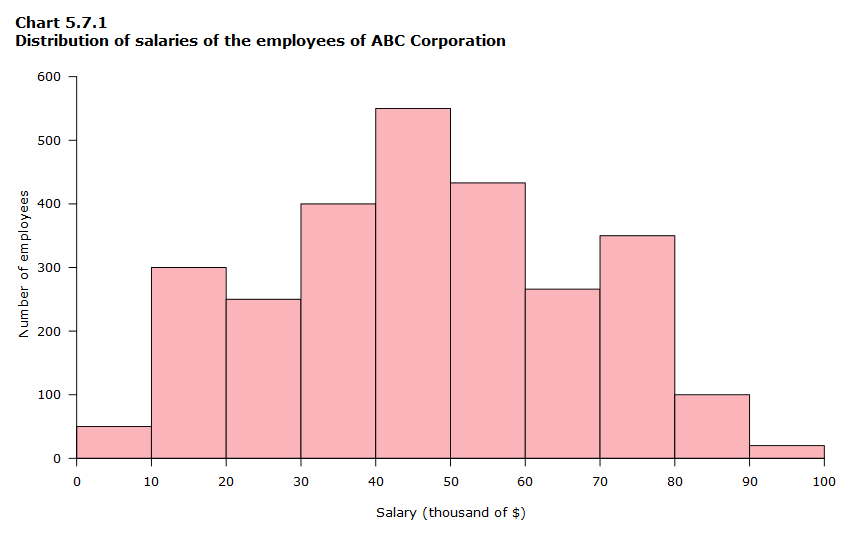
\includegraphics[width=0.7\textwidth]{1}
			            \end{center}
			            \caption{An example histogram}\label{fig:1}
		            \end{figure}
	      \end{itemize}
\end{itemize}

\subsection*{Probability Plots}
\begin{itemize}
	\item For smaller sample sizes, histograms are not as effective, so
	      a graphical method we can use instead is probability plots.
	      \begin{itemize}
		      \item A \textbf{probability plot }is used to confirm a hypothesis about
		            whether or not some data follows a certain distribution.
	      \end{itemize}
	\item A worked example of how to use a probabiltity plot to confirm if some
	      data has a normal distribution:
	      \begin{enumerate}
		      \item Suppose we have some data, which can be found in the table below:
		            \begin{center}
			            \begin{tabular}{c}
				            Observed Length of Fish \\
				            \hline
				            100                     \\
				            98                      \\
				            101                     \\
				            93                      \\
				            123                     \\
				            112                     \\
				            85                      \\
				            76                      \\
				            119                     \\
				            111                     \\
			            \end{tabular}
		            \end{center}
		      \item Sort the data in ascending order:
		            \begin{center}
			            \begin{tabular}{c}
				            Observed Length of Fish \\
				            \hline
				            76                      \\
				            85                      \\
				            93                      \\
				            98                      \\
				            100                     \\
				            101                     \\
				            111                     \\
				            112                     \\
				            119                     \\
				            123
			            \end{tabular}
		            \end{center}
		      \item Number the data from index 1 to 10:
		            \begin{center}
			            \begin{tabular}{c | c}
				            Number (i) & Observed Length of Fish \\
				            \hline
				            1          & 76                      \\
				            2          & 85                      \\
				            3          & 93                      \\
				            4          & 98                      \\
				            5          & 100                     \\
				            6          & 101                     \\
				            7          & 111                     \\
				            8          & 112                     \\
				            9          & 119                     \\
				            10         & 123
			            \end{tabular}
		            \end{center}

		      \item For each index, calculate the ``Expected Cumulative
		            Probability'', which follows the formula $\frac{i - 0.5}{n}$,
		            where $i$ is the index in question and $n$ is the total data
		            points:
		            \begin{center}
			            \begin{tabular}{c | c | c}
				            Number (i) & Observed Length of Fish & Expected Cumulative Probability \\
				            \hline
				            1          & 76                      & 0.05                            \\
				            2          & 85                      & 0.15                            \\
				            3          & 93                      & 0.25                            \\
				            4          & 98                      & 0.35                            \\
				            5          & 100                     & 0.45                            \\
				            6          & 101                     & 0.55                            \\
				            7          & 111                     & 0.65                            \\
				            8          & 112                     & 0.75                            \\
				            9          & 119                     & 0.85                            \\
				            10         & 123                     & 0.95
			            \end{tabular}
		            \end{center}
		      \item Determine the $z$-scores (or $z$-value) for each expected cumulative
		            probability from the standard normal probability
		            distribution (which is a normal probability distribution
		            with $\mu = 0$ and $\sigma = 1$). That is, you need to find which
		            $z$-score will give you the expected cumulative probability in question.
		            Some notes about $z$-scores before the table containing the
		            $z$-scores for cumulative probabilities in this example:
		            \begin{itemize}
			            \item A $z$-score/value is a statistical measurement
			                  that describes the value's relationship to the mean
			                  of a group of values. $z$-scores are
			                  measured in terms of ``standard deviations from the
			                  mean.'' For example, if a value of the random
			                  variable $X = x$ has a $z$-score of $1$, it means that
			                  the value of $X = x$ is 1 standard deviation to the
			                  right of the mean.
			            \item \emph{(Not useful for this example but useful to
				                  know in general)} Given a value $X = x$, a
			                  $z$-score for a normal distribution can be
			                  calculated with the following formula (where
			                  $\mu$ is the mean, and $\sigma$ is the standard
			                  deviation of the
			                  distribution):
			                  \[
				                  z = \frac{x - \mu}{\sigma}
			                  \]
			            \item \emph{(Somewhat useful for this example)} Given a $z$-value,
			                  if you want to find the area to the left of that
			                  $z$ value (essentially area to the left of $z$ standard
			                  deviations from the mean), you can use a
			                  \textbf{Z lookup table} (which would have to be
			                  provided to us, see
			                  \href{https://www.ztable.net/}{this link}) for
			                  information.
			            \item \emph{(Directly useful for this example)}: in this case,
			                  we want to find the opposite of the above point; we want to
			                  find the $z$ \emph{given} the area to the left of the $z$-score
			                  (the Expected Cumulative Probability). We can do this in one of
			                  two ways:
			                  \begin{itemize}
				                  \item Use the \emph{normal distribution's quantile function} (very complicated, would not even bother looking it up)
				                  \item Use the \emph{Z lookup table, but backwards}
				                  \item (Recommended) Use software, namely the \verb|qnorm| function from R, which does exactly what we want.
			                  \end{itemize}
		            \end{itemize}
	      \end{enumerate}
\end{itemize}

Plugging in each Expected Cumulative Probability into \verb|qnorm|:
\begin{center}
	\begin{tabular}{c | c | c | c}
		Number (i) & Observed Length of Fish & Expected Cumulative Probability & Z-Scores (approx) \\
		\hline
		1          & 76                      & 0.05                            & -1.64             \\
		2          & 85                      & 0.15                            & -1.03             \\
		3          & 93                      & 0.25                            & -0.67             \\
		4          & 98                      & 0.35                            & -0.39             \\
		5          & 100                     & 0.45                            & -0.13             \\
		6          & 101                     & 0.55                            & 0.13              \\
		7          & 111                     & 0.65                            & 0.38              \\
		8          & 112                     & 0.75                            & 0.67              \\
		9          & 119                     & 0.85                            & 1.04              \\
		10         & 123                     & 0.95                            & 1.64
	\end{tabular}
\end{center}
\begin{itemize}
	\begin{enumerate}
		\item[6.] Plot the points $(x, y)$, where $x$ is the Observed Length of Fish and $y$ is the associated $z$-score.
			This plot is a \textbf{normal probability plot}. If the points fall roughly in a straight line, you can
			assume you have a normal distribution, and your initial hypothesis is correct.
	\end{enumerate}
	\item For my sanity and yours, I will not include examples for more complicated
	      distributions (like exponential, etc.). They are extremely hard to find
	      and I doubt we will be tested on them because normal probability plots
	      are hard enough.
\end{itemize}

\section*{Simulating Realizations of Random Variables with the Uniform
  Distribution}

Consider the following theorem:

\begin{theorem}
	[Inverse Transform Method] Suppose $X$ is a countinuous random
	variable with CDF $F$, where $F$ is invertible with inverse function
	$F^{-1}$. Let $U \tilde Unif(0, 1)$. Then the distribution of $F^{-1}(U)$
	is equal to the distribution of $X$.
\end{theorem}


\end{document}
